\section{Dynsem Evaluation Strategy}
\label{sec:dynsem-eval-strat}
An implementation for the \texttt{IEvaluationStrategy} as discussed in
\cref{sec:eval-strat} has been made for languages that specify their dynamic
semantics using DynSem. The implementation class, called
\texttt{``DynSemEvaluationStrategy''} (see \cref{fig:uml-dynsem-eval-strat}),
evaluates REPL-specific DynSem rules and maintains the environment in which
evaluation takes place.

This section first goes over the configuration interface for DynSem that is
provided by the REPL. After that, the implementation of DynSem and of the
evaluation strategy are discussed in more detail.

\subsection{The REPL configuration interface}
\label{sec:impl-repl-spec}
To evaluate a program in their language within the REPL, the language designer
has to make two sorts of configurations for the REPL in their DynSem
specification. The first is a rule for initializing the execution environment
for the REPL, shown in \cref{lst:shell-init}. The second are the rules for
implementing the REPL-specific semantics as discussed in
\cref{ssec:repl-spec-semant}.

\paragraph{Environment initialization} The initialization rule shown in
\cref{lst:shell-init} is evaluated upon the initialization of the evaluation
strategy. It instantiates the semantic components that forms the execution
environment for the REPL: an environment with an initial variable binding of
$x \mapsto 4$, and an empty store. The evaluation strategy uses this in its
successive evaluations, and updates the execution environment after each result.

\begin{minipage}{\textwidth}
\begin{lstlisting}[language=dynsem,caption={The initialization rule for the
semantic components},label={lst:shell-init},numbers=left]
rules
  // Initialization of shell state: an environment with "x" bound to 4,
  // and an empty store.
  ShellInit() -init-> ShellInit() :: Env { "x" |--> NumV(4) }, Store {}.
\end{lstlisting}
\end{minipage}

\paragraph{REPL-specific semantics} The second kind of configuration are the
rules for the REPL-specific semantics. These can be seen as entry points for the
REPL to the interpreter. The rules are all named ``shell'', so that they are
distinct of the ordinary semantics. \Cref{lst:shell-rule} shows an example of
such a rule. The rule implements a construct that is only valid when evaluating
within the REPL: it implements binding the result of an expression to a
variable. With the specification of this rule, the bound variable can be used in
successive evaluations done by the user.

Note that the environment \textit{E} is passed as a read-write component,
instead of a read-only component as is explained in \cref{ssec:dynsem}. This is
because in this case the environment \emph{should} be writable, since the
resulting environment after execution should be available to the REPL. Note also
that in line 5 of the rule, the rest of the specification is recursively
invoked. This shows that much of the existing specification can be reused when
implementing the REPL-specific semantics.

\begin{minipage}{\textwidth}
\begin{lstlisting}[language=dynsem,caption={A rule specifying semantics specific
to the REPL.},label={lst:shell-rule},numbers=left]
rules
  // let x = 2
  Let(x, e) :: E -shell-> v :: E'
  where
    E |- e :: Store {} --> v :: Store _;
    E |- bindVar(x, v) --> E'.
\end{lstlisting}
\end{minipage}

\subsection{The implementation}
\label{sec:implementation}

\begin{figure}[h]
  \centering
  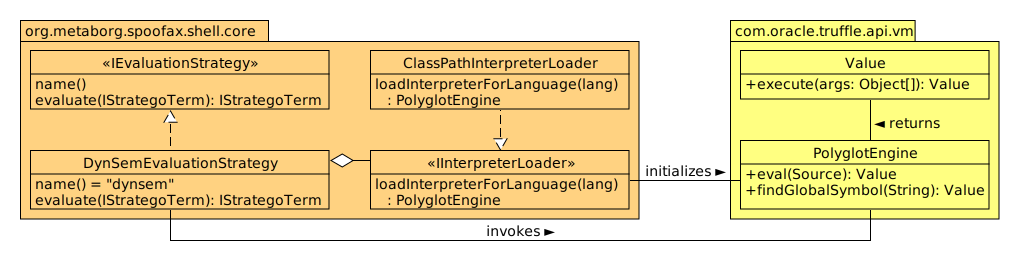
\includegraphics[width=0.8\textwidth]{uml-dynsem-eval-strat}
  \caption{UML diagram of the \texttt{DynSemEvaluationStrategy} and its
    collaborators.}
  \label{fig:uml-dynsem-eval-strat}
\end{figure}

%%% Local Variables:
%%% mode: latex
%%% TeX-master: "../main"
%%% End:
